\chapter{The Visual Atlas of Composition Mosaics}
\label{chap:visual-atlas}

\section*{Cartographic Conventions}

This visual catalogue displays the complete combinatorial census of all $509$ non-equivalent dihedral composition mosaics across the circular rings $\mathbb{Z}_1$ through $\mathbb{Z}_8$, ordered canonically by lattice ring order $n$, part count $s$, partition shape $\lambda \vdash n$, and intra-shape invariants.

Each drawing portrays an individual dihedral orbit through its canonical representative inscribed in a regular $n$-gon:
\begin{itemize}
    \item \textbf{Lattice Frame}: The $n$ vertices of $\mathbb{Z}_n$ are oriented with vertex $0$ at the zenith, advancing clockwise $0, 1, \dots, n-1$. A regular $n$-gon is lightly delineated in the background to establish the metric frame (for $n=1$, a circular boundary; for $n=2$, a dashed line of vertices).
    \item \textbf{Block Delineation}:
    \begin{itemize}
        \item \emph{Unigons ($d=1$)} are marked by circular nodes at the corresponding lattice vertex.
        \item \emph{Digons ($d=2$)} are drawn as prominent straight metric chords connecting the vertex pair.
        \item \emph{Inscribed Polygons ($d \ge 3$)} are drawn as shaded polygonal tiles bounded by their cyclic perimeter chords.
    \end{itemize}
    \item \textbf{Bilateral Symmetry Colouring}:
    \begin{itemize}
        \item \textbf{Blue}: Bilaterally symmetric (achiral) blocks possessing an internal axis of dihedral reflection.
        \item \textbf{Pink}: Scalene (chiral) blocks lacking reflection symmetry.
    \end{itemize}
    \item \textbf{Orbit Invariants}:
    \begin{itemize}
        \item \textbf{Upper-Left Index}: Bold ring-local integer identifier ($1 \dots M_n$) referencing the master catalogue in Section~\ref{sec:relational-datasets} and \path{data/mosaics.tsv}.
        \item \textbf{Lower-Right Orbit Size}: Dihedral orbit length $|\mathcal{O}| \in \{1, \dots, |D_n|\}$ under the action of $D_n$.
    \end{itemize}
\end{itemize}

\clearpage
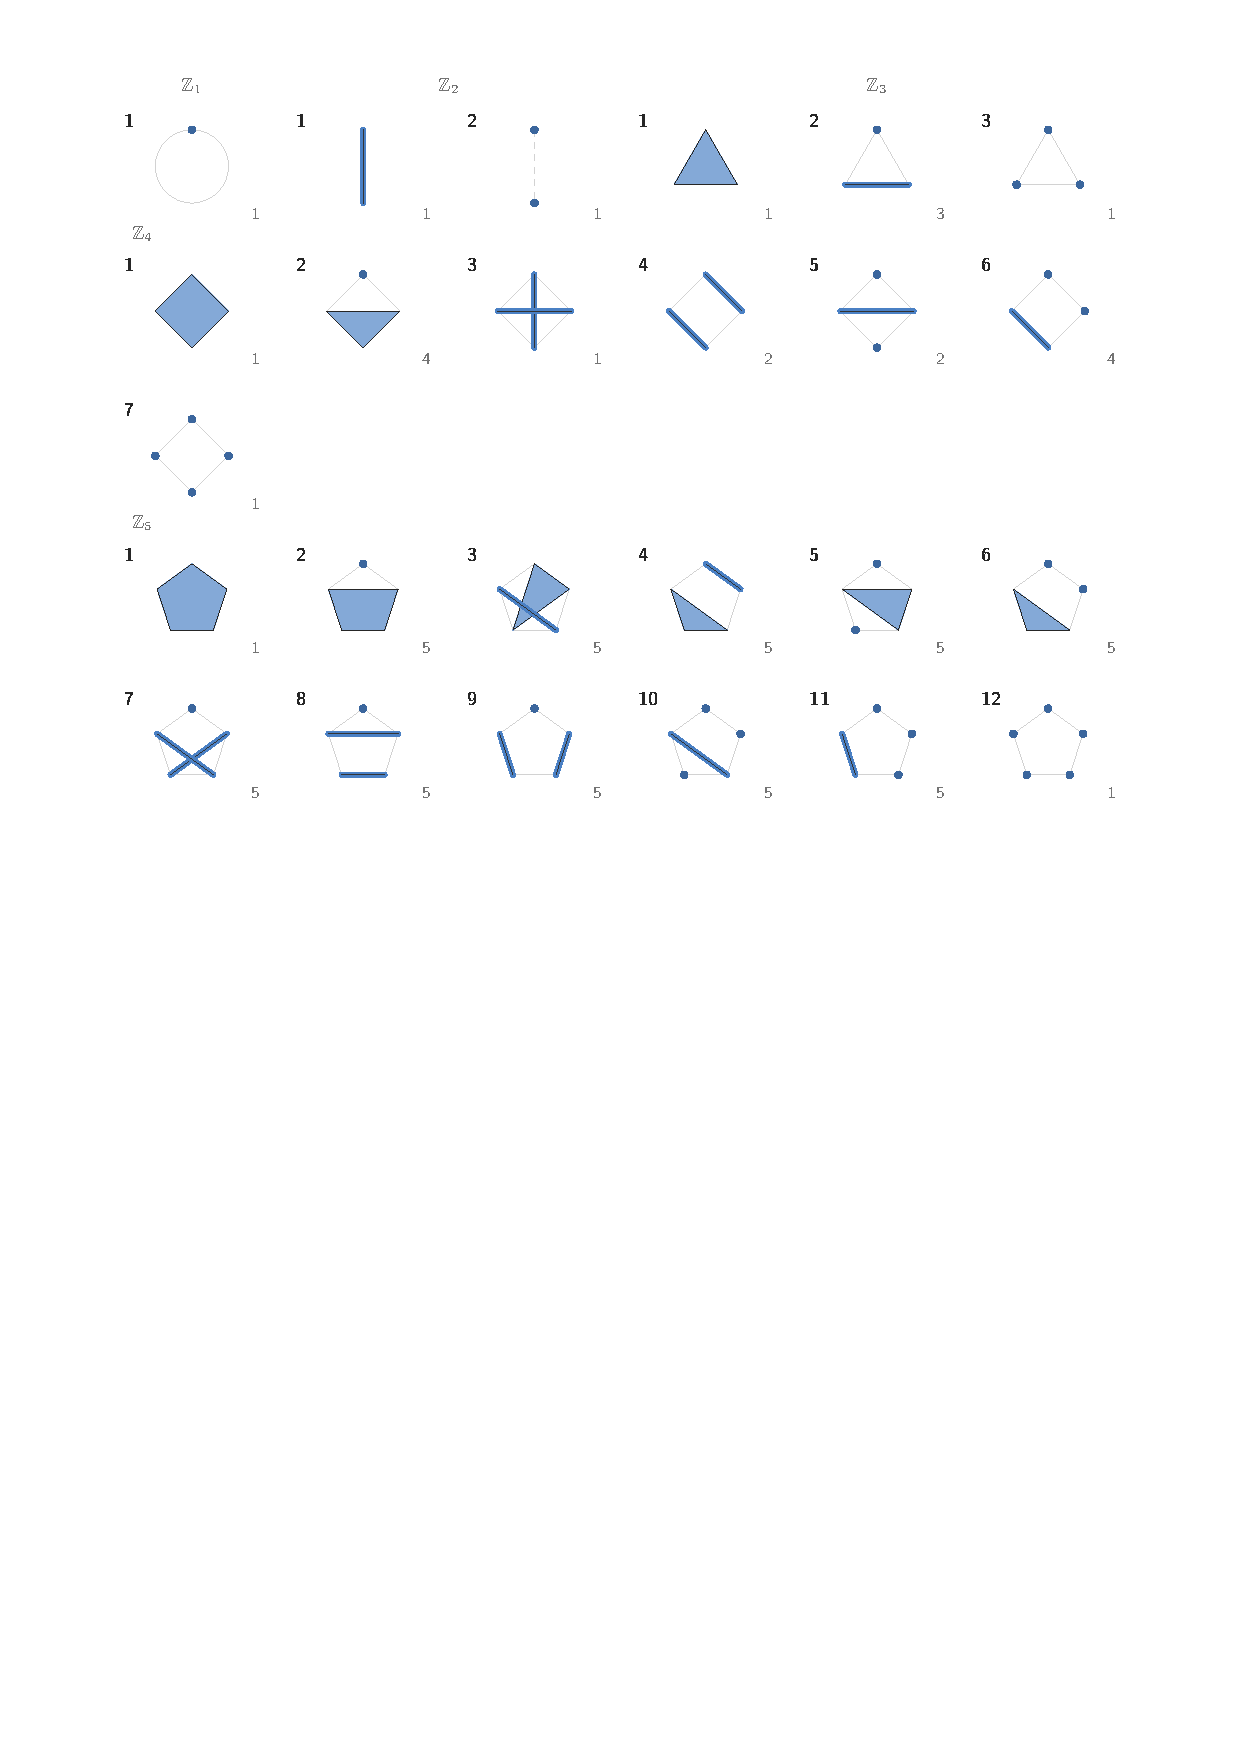
\includepdf[
  pages=-,
  offset=0 -16mm,
  pagecommand={\thispagestyle{headings}},
  addtotoc={
     1, section, 1, {The Small Cyclic Lattices \texorpdfstring{($\mathbb{Z}_1$ through $\mathbb{Z}_5$)}{}}, sec:ring-z1-z5,
     2, section, 1, {The Hexagonal Lattice \texorpdfstring{$\mathbb{Z}_6$}{Z6}}, sec:ring-z6,
     3, section, 1, {The Heptagonal Lattice \texorpdfstring{$\mathbb{Z}_7$}{Z7}}, sec:ring-z7,
     5, section, 1, {The Octagonal Lattice \texorpdfstring{$\mathbb{Z}_8$}{Z8}}, sec:ring-z8
  }
]{plates/plates_z1_z8.pdf}
